\documentclass{beamer}
\usepackage[english]{babel} 
\usepackage[latin1]{inputenc} 
\usepackage{amsthm}
\usepackage{dsfont}
\usepackage{xcolor}
\usepackage{multimedia}
 
\title{Preprocessing and Classification of ERD/ERS Signals}
%\subtitle{Untertitel}
\author{Florian Eichin}
\institute{Freiburg University}
\date{\today}

\usetheme{metropolis}

\selectlanguage{english}

 
\begin{document}

\maketitle

\begin{frame}
	\frametitle{Contents}
	\tableofcontents
\end{frame}

\section{How do we measure brain activity?}

\begin{frame}
\frametitle{How do we measure brain activity?}
	\begin{itemize}
	\item measure the electromagnetical effects of brain processes
	\item in this talk: via EEG-electrodes on the scalp
	\end{itemize}
	\centering
	\includegraphics[scale=0.26]{kappe.jpg} \\
	{\tiny [Wolpaw, 2011]}
\end{frame}


\begin{frame}
	\frametitle{Representation of EEG-Signals}
	\begin{definition}
	With $x: \mathds{N} \rightarrow \mathds{R}^n$, we call $x(t)$ the {\bf sample at timepoint} $t$. \\
	For $t, u \in \mathds{N}$ the matrix
	\begin{equation}
		X = (x(t), x(t+1), ..., x(t+u))
	\end{equation} 
	is the {\bf epoch} at timepoint $t$ with length $u$.
	\end{definition}
	\centering
	\includegraphics[scale=0.15]{waves.png}
\end{frame}

\begin{frame}
\frametitle{Frequency Spectrum}
\centering
\includegraphics[scale=0.30]{spectrum_red.png}
	\begin{itemize}
	\item Our signal consists of a composition electromagnetical waves
	\item it might be a good idea to have a look at the frequency-bands to gain information about the underlying processes
	\end{itemize}
\end{frame}

\section{Oscillatory Analysis: Neurological Background}

\begin{frame}
\frametitle{Pyramidal Cells}
	\begin{itemize}
	\item largest contributor to the electromagnetical activity we can  measure from the outside
	\item aligned orthogonally to the scalp on the surface of the brain
	\end{itemize}
	\centering
	\includegraphics[scale=0.26]{pyramidal.png}
	\includegraphics[scale=0.25]{pyramidal_aligned.jpg}	\\
	{\tiny [W-CH Lee, 2006 and Aarhuus University, 2004]}
\end{frame}

\begin{frame}
\frametitle{Event Related (De)Synchronisations}
	Whenever certain populations of neurons are inactive, they enter an {\bf idle state}, synchronously oscillating at characteristic frequencies:
	\begin{itemize}
		\item $\alpha$- / $\mu$-rhythms: 8-15 Hz mostly found in the visual / motor and sensory cortex
		\item $\beta$-rhythm: 16-31 Hz, sensory and motor cortex	
	\end{itemize}	
	\centering
	\movie[]{\includegraphics[scale=0.15]{video_start.png}}{alpha.mp4} \\
	{\tiny [Backyard Brains, 2014]}
\end{frame}

\begin{frame}
\frametitle{Event Related (De)Synchronisations}
	\begin{itemize}
	\item parts of the brain are linked to certain tasks
	
	\item local ERD/ERS might help us classify between left and right movement 
	\end{itemize}
	\centering
	\includegraphics[scale=0.27]{head.png}
	{\tiny [Blankertz, 2008]}
\end{frame}



\section{What are the challenges?}

\begin{frame}
\frametitle{Noise and Artifacts}
Our channels are usually not only picking up relevant neuronal activity, our signal is obscured by
	\begin{itemize}
	\item {\bf Artifacts}: 
	\begin{itemize}
	\item environmental (power lines, electric devices, ...)
	\item from BCI-hardware (amplifier, cables, electrodes, ...)
	\item from the body (muscle contractions, blood flow, ...)
	\end{itemize}
	\item {\bf Noise} (from unrelated brain activity)
	\end{itemize}
\end{frame}

\begin{frame}
\frametitle{Dimensionality}
	\begin{itemize}
	\item EEG-data has lots of {\bf dimensions} (usually up to 128 channels) with lots of redundancy encoded
	\item the more dimensions we want to use for classification, the more data we need
	\item we usually only have the data from one session, that we can use for training our BCI
	\end{itemize}
	\includegraphics[scale=0.22]{cap.jpg}
	\includegraphics[scale=0.14]{waves.png}
	{\tiny [University of Nebraska, 2013]}	
	%TODO: search numbers of increase aat LDA
	%TODO: LDA picture instead of waves?
\end{frame}


\section{A simple approach: Laplace Filters}


\begin{frame}
	\frametitle{Filters}
	\begin{definition}
	A {\bf filter} is a linear projection $w: \mathds{R}^n \rightarrow \mathds{R}$ where $n$ is the number of channels. We obtain the 
	filtered signal by calculating:
	\begin{equation}
		x_w(t) = w \cdot x(t)
	\end{equation}
	The $w_i$ are called {\bf weights}. Note that filters can be simultianiously applied by multiplying with a 			{\bf filter matrix} $W$, where each row vector is a filter:
	\begin{equation}
		x_W(t) = W \cdot x(t)
	\end{equation} 
	\end{definition}
\end{frame}

\begin{frame}
\begin{center}
	\frametitle{Laplace Filters}
	\includegraphics[scale=0.265]{lfilter1.png}
\end{center}
\end{frame}

\begin{frame}
	\begin{center}
	\frametitle{Laplace Filters}
	\includegraphics[scale=0.265]{lfilter1.png}
	\end{center}
	$x(t) = (x_1(t), ..., x_9(t))$ 
\end{frame}

\begin{frame}
	\begin{center}
	\frametitle{Laplace Filters}
	\includegraphics[scale=0.265]{lfilter2.png}
	\end{center}
	$x(t) = (x_1(t), ..., x_9(t))$ 
\end{frame}

\begin{frame}
	\begin{center}
	\frametitle{Laplace Filters}
	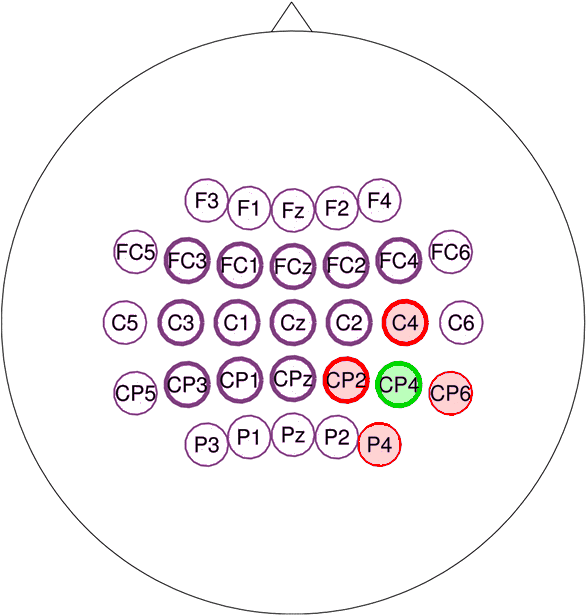
\includegraphics[scale=0.265]{lfilter3.png}
	\end{center}
	$x(t) = (x_1(t), ..., x_9(t))$ 
\end{frame}

\begin{frame}
	\begin{center}
	\frametitle{Laplace Filters}
	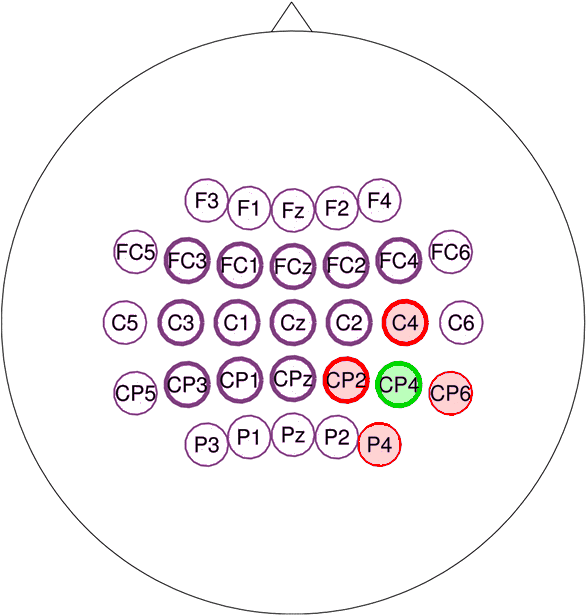
\includegraphics[scale=0.265]{lfilter3.png}
	\end{center}
	$x(t) = (x_1(t), ..., x_9(t))$ \\
	$w = (0, ..., 0, \textcolor{red}{-\frac{1}{3}}, \textcolor{red}{-\frac{1}{3}}, 
	\textcolor{red}{-\frac{1}{3}}, \textcolor{green}{1})$ 
\end{frame}


\begin{frame}
	\begin{center}
	\frametitle{Laplace Filters}
	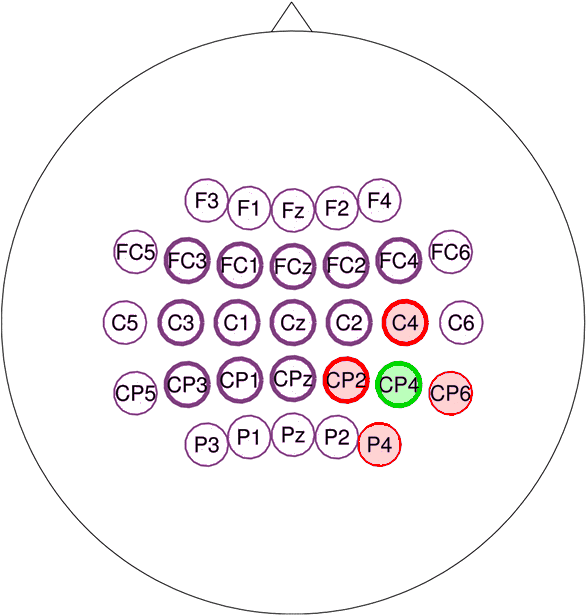
\includegraphics[scale=0.265]{lfilter3.png}
	\end{center}
	$x(t) = (x_1(t), ..., x_9(t))$ \\
	$w = (0, ..., 0, \textcolor{red}{-\frac{1}{3}}, \textcolor{red}{-\frac{1}{3}}, 
	\textcolor{red}{-\frac{1}{3}}, \textcolor{green}{1})$ \\
	$x_w(t) = w \cdot x(t) =  \textcolor{red}{-\frac{1}{3} \cdot (x_6 + x_7 + x_8)} + \textcolor{green}{x_9}$
\end{frame}


\section{More sophisticated: Common Spacial Patterns (CSP)}

\begin{frame}
	\frametitle{Common Spacial Patterns}
	\begin{itemize}
	\item an algorithm, that learns filters from collections of data sample epochs $X_i \in \mathds{R}^{NxC}$ for classes $1$ and $-1$
	\item idea: {\bf variance optimisation} between the two classes
	\end{itemize}
	\includegraphics[scale=0.3]{scatter.png}
	\includegraphics[scale=0.3]{scatter_csp.png}
\end{frame}

\begin{frame}
	\frametitle{Covariance Estimation}
	Let $X_1, ..., X_k \in \mathds{R}^{NxC}$ be the samples for class $c$. Then we estimate the {\bf covariance matrix} by
	\begin{equation}
		\Sigma_c = \frac{1}{k} \sum_{i=1}^{k}X_i^T X_i
	\end{equation} 
\end{frame}



\begin{frame}
	\frametitle{Covariance Optimisation}
	\begin{itemize}
	\item Let $\Sigma_{+}, \Sigma_{-} \in \mathds{R}^{CxC}$ be the covariance matrix for class 1 / -1
	\item Subsequently find orthogonal vectors $w_i$ that satisfy
	\begin{equation}
		w_i = argmax_{w \in \mathds{R}^{n*}} \frac{w \Sigma_{+} w^T}{w \Sigma_{-} w^T}
	\end{equation}
	\item the obtained $W$ will project our data into a space, where the first (last) coordinate refers to the feature
	that has the highest variance for class 1 (-1)
	\end{itemize}
\end{frame}


\begin{frame}
	\frametitle{Analytical Solution}
	\begin{itemize}
	\item A solution for $W$ can also be obtained by solving
	\begin{equation}
		w \Sigma_+ = \lambda \cdot w \Sigma_-
	\end{equation}
	\item the eigenvecors $w_1, ..., w_n$ with eigenvalues $\lambda_1 > \lambda_2 >...> \lambda_n$ yield $W = (w_1, ..., w_n)^T$
	\item $\lambda_i$ corresponds to the amount of variance in coordinate $i$ in our surrogate space
	\end{itemize}
	%TODO: Add Herleitung for Eigenvalue problem
	%TODO: Add intuition
\end{frame}

\begin{frame}
	\frametitle{Forward and Backward Model}
	\begin{definition}
	$W$ is also called {\bf backward model},
	$A = W^{-1}$ the {\bf forward model}.
	\end{definition}
	
	\includegraphics[scale=0.328]{topo_filters.png}
	\includegraphics[scale=0.328]{topo_patterns.png}
	% Intuition behind f and bf model
	%Topological Maps
\end{frame}

\begin{frame}
\frametitle{Relation to Principal Component Analysis}
	CSP is a {\bf supervised generalization} of PCA for two classes. \\
	If class -1 is is uncorrelated, CSP yields the same filter matrix as PCA for class 1.
	
	\begin{proof}
	Let $\Sigma_{+}$ and $\Sigma_{-}$ be the covariance matrices for class 1 and -1. \\
	Then $\Sigma_{-} = I$ and we have 
	\begin{equation}
	w_i = argmax_{w \in \mathds{R}^{n*}} \frac{w \Sigma_{+} w^T}{w \Sigma_{-} w^T} = argmax_{w \in \mathds{R}^{n*}} \frac{w \Sigma_{+} w^T}{w w^T}
	\end{equation}
	which is the optimization criterion for PCA.
	\end{proof}		
	
	
\end{frame}

\section{How good is it?}

\begin{frame}
\frametitle{Noise Reduction and Dimensionality}
	\begin{itemize}
	\item CSP implements noise reduction and lower dimensionality
	\item $\alpha$- and $\beta$-bands are more prominent in the {\color{blue}target epochs} after applying filters yielding an opportunity to discriminate from the {\color{red}non-target} epochs
	\end{itemize}
	\centering
	\includegraphics[scale=0.29]{spectrum_before.png}
	\includegraphics[scale=0.29]{spectrum_after.png}
\end{frame}

\begin{frame}
\frametitle{Application}
Widely used among other methods such as PCA and ICA
\begin{itemize}
	\item Easy to use and implement
	\item Low runtime, just a linear mapping
	\end{itemize}
On the other hand:
	\begin{itemize}
	\item Hyperparameters (length, timepoint of sample epochs)
	\item supervised: need for labelled data
	\item need for training data beforehand
	\end{itemize}
\end{frame}

\begin{frame}
\frametitle{Sources}
\begin{itemize}
	\item Wolpaw, Brain-Computer Interfaces: principles and practice. Oxford Univ. Press, 2011.
	\item Blankertz B, Tomioka R, Lemm S, Kawanabe M, Müller KR, Optimizing Spatial Filters for Robust EEG Single-Trial Analysis. IEEE Signal Process Mag, 25(1):41-56, 2008.
	\item mne$\-$tools.github.io/dev/auto$\_$examples/decoding/ \\ plot$\_$decoding$\_$csp$\_$eeg.html
	\item Schalk, G McFarland, DJ Hinterberger T, Birbaumer N, Wolpaw JR, BCI2000: A General-Purpose Brain-Computer Interface (BCI) System. IEEE TBME 51(6):1034-1043, 2004

\end{itemize}
\end{frame}

\end{document}